\section{}


\begin{center}
	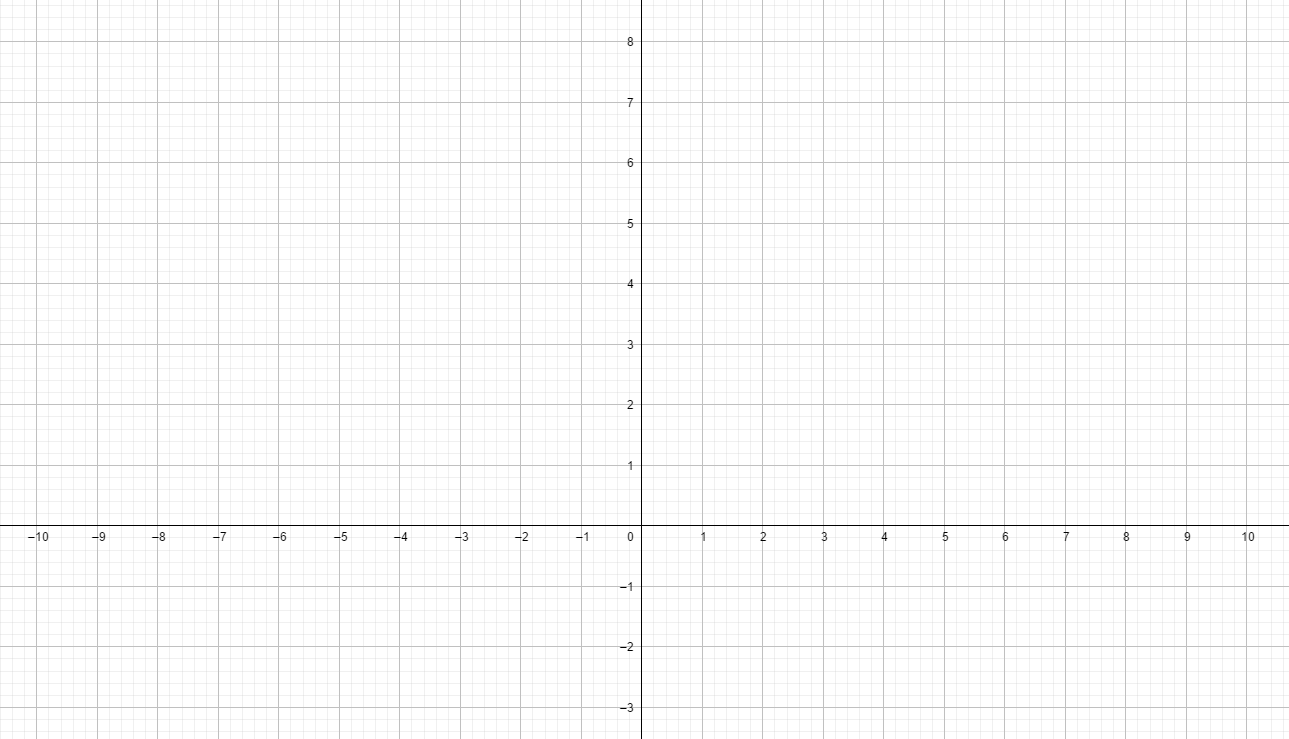
\includegraphics[scale=0.5]{vide}
\end{center}
\begin{questions}
	
	
	
	\question[2] Tracer la droite correspondant à la fonction $f(x) = -2x + 3$
	
	
	\fillwithdottedlines{3cm}
	
	\question[2]Tracer la droite d'équation $ y  = \frac{1}{2}x - 1$
%	
	\fillwithdottedlines{3cm}
	
	\question[2] Tracer la droite de coefficient directeur $a = 2$ passant par le point $B(-8; -2)$.
	

\end{questions}

\section{}

\begin{center}
	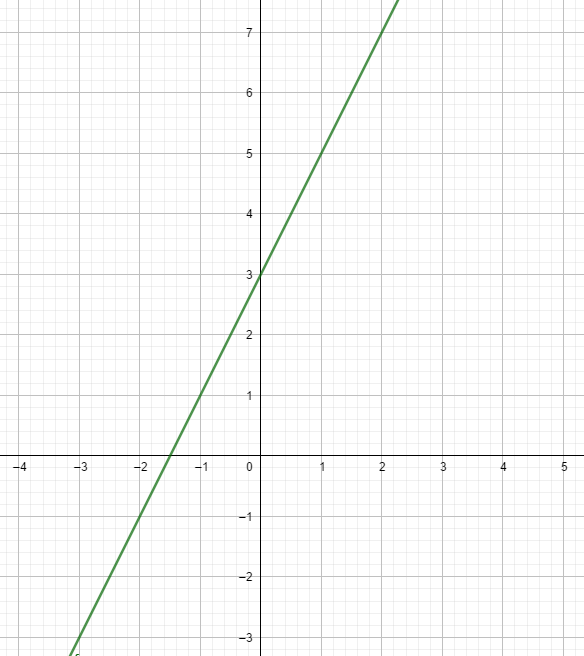
\includegraphics[scale=0.5]{fct1}
	
\end{center}

\begin{questions}
	\question[2] Déterminer la fonction représentée par la droite ci-dessus.
	\fillwithdottedlines{7cm}
	
	\question[2] Déterminer par la calcul si le point $M(2; 7)$ appartient à la droite.
	
	\fillwithdottedlines{4cm}
\end{questions}

\label{LastPage}